\subsection{Программный пакет \texttt{nudisxs}}

\texttt{nudisxs}~\cite{nudisxs2022} — программный модуль на языке Python~3, предназначенный для вычисления сечений нейтрино–нуклонного взаимодействия в области глубоконеупругого рассеяния по формуле~\eqref{eq:xsec_general}. 
Его вычислительное ядро основано на пакете \texttt{XsDis}, написанном на языке \texttt{Fortran-77} В.~А.~Наумовым и К.~С.~Кузьминым. 
В отличие от функционала \texttt{XsDis}, использующего фиксированный набор партонных функций, пакет \texttt{nudisxs} обеспечивает динамическое подключение партонных распределений из библиотеки \texttt{LHAPDF6}~\cite{aartsenLHAPDF2020}.

\texttt{nudisxs} позволяет вычислять дважды дифференциальные сечения $d^2\sigma/dx dy$, дифференциальные сечения по одной переменной и полные сечения взаимодействия в широком диапазоне энергий — от сотен~МэВ до~$10^{15}$~ГэВ. 
Он предназначен для задач нейтринной астрофизики и моделирования событий в нейтринных телескопах и может быть легко интегрирован в существующие исследовательские проекты.

Реализация использует библиотеки \texttt{NumPy}~\cite{2020NumPy-Array}, \texttt{SciPy}~\cite{2020SciPy-NMeth} и \texttt{vegas}~\cite{lepageVegas2021} для многомерного Монте–Карло интегрирования, что обеспечивает высокую производительность и удобство при численном анализе и тестировании. 
%

Логическая архитектура пакета \texttt{nudisxs} показана на рис.~\ref{fig:nudisxs1}. 
Основой расчётов является загрузка партонных функций из библиотеки \texttt{LHAPDF6}, используемых для построения структурных функций $F_i(x, Q^2)$, входящих в выражение~\eqref{eq:xsec_general}. 
Пользовательский интерфейс реализован в модуле \texttt{dis}, где задаются тип лептона (нейтрино или антинейтрино), мишень (протон, нейтрон или изоскаляр), энергия нейтрино, минимальное значение $Q^2$, а также выбранный набор партонных распределений и параметров модели. 
Вычисление дважды дифференциальных сечений для заряженного и нейтрального токов выполняют модули \texttt{xs\_cc} и \texttt{xs\_nc}. 
Часть исходного кода, написанного на~\texttt{Fortran-77}, доступна через интерфейс \texttt{f2py} и обеспечивает быстрые, проверенные временем вычисления ключевых выражений. 
Интерполяция партонных распределений, построение структурных функций и численные процедуры реализованы средствами \texttt{SciPy}.

\begin{figure}[!h]
\centering
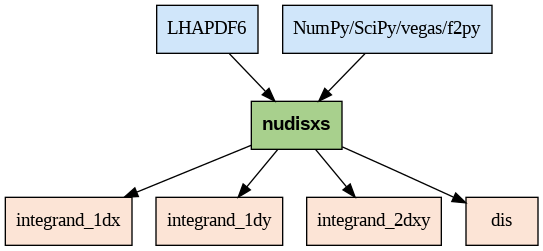
\includegraphics[width=\linewidth]{images/nudisxs_diagram.png}
\caption{Структура программного пакета \texttt{nudisxs} и его зависимости.}
\label{fig:nudisxs1}
\end{figure}

Пакет \texttt{nudisxs} распространяется через платформу \texttt{PyPI} как открытое программное обеспечение. 
Он легко устанавливается и интегрируется в существующие симуляционные цепочки. 
В рамках настоящей работы для расчёта сечений использовуется \texttt{nudisxs}.
